% am121 LaTeX template, for assignment and extreme optimization writeups
% created by Chris Coey for am121 Spring 2012

\documentclass[12pt]{article}
% packages
\usepackage{amssymb,amsmath,amsthm} 
\usepackage[margin=.90in]{geometry}
\usepackage{graphicx,ctable,booktabs}
% begin paragraphs on empty line rather than indent
\usepackage[parfill]{parskip}
% Allow line wrapping 
\usepackage{listings}
\usepackage{float}
\lstset{
basicstyle=\small\ttfamily,
columns=flexible,
breaklines=true
}
% eps to pdf, declare graphics
\usepackage{epstopdf}
\DeclareGraphicsRule{.tif}{png}{.png}{`convert #1 `dirname #1`/`basename #1 .tif`.png}
% enable highlighting text: use \hl{your text here}
\usepackage{soul}

% adjust section and subsection labelling 
\def\thesection{\arabic{section}}
\def\thesubsection{\arabic{section}.\arabic{subsection}}
\makeatletter
% section as task
\newenvironment{task}{\@startsection
       {section}{1}
       {0.4em}{-.5ex plus -1ex minus -.2ex}{.5ex plus .2ex}
       {\pagebreak[3]\large\bf\noindent{Task}}}
       {\nopagebreak[3]\vspace{3ex}\begin{center}\rule{1\linewidth}{.3pt}\end{center}}
% subsection as subtask
\newenvironment{subtask}{\@startsection
       {subsection}{2}
       {0.3em}{0ex plus -1ex minus -.2ex}{.5ex plus .2ex}
       {\pagebreak[3]\large}}
       {\nopagebreak[3]\vspace{3ex}\begin{center}\rule{0.5\linewidth}{.3pt}\end{center}}
\makeatother

% headers
\usepackage{fancyhdr}
\pagestyle{fancy}
\chead{} 
\rhead{\thepage} 
% footer
\lfoot{\small\scshape AM121/ES121} 
\cfoot{} 
%%%% insert your name here %%%%
\rfoot{\footnotesize Jeremy Nixon, Millie Shi,  David Freed,  Chris Bruno} 
\renewcommand{\headrulewidth}{.3pt} 
\renewcommand{\footrulewidth}{.3pt}
\setlength\voffset{-0.25in}
\setlength\textheight{648pt}

\begin{document}
%%%% change homework number here %%%%
\title{AM121/ES121: Extreme Optimization}
%%%% insert your name and TF's name here %%%%
\author{Millie Shi\\ Jeremy Nixon \\ David Freed \\ Chris Bruno }
\date{\today}   
\maketitle
\thispagestyle{empty}
\bigskip

%%%%%%%%%%%%%%%%%%%%%%%%%%%%%%%
% task 1
\begin{task}{The Mathematical Formulation}
\begin{enumerate}
\item To deduce our optimal objective function, we considered the actual problem at hand. We are trying to cure a patient of a tumor while balancing two objectives: maximizing the radiation aimed at the tumor and minimizing the radiation aimed at the critical area. We chose minimizing the radiation aimed at the critical area as our objective function because we want to discourage any responses that would have substantial radiation aimed at the critical area. The ultimate goal is improving the health of the patient and any solution which kills the tumor but results in a severe health reduction to the patient, or even death, is not a viable solution. 

Thus our objective just minimizes radiation aimed at the critical area, which we defined before.  

\begin{eqnarray*}  
 \textrm{Sets} &  R & \textrm{The set of rows} \\
			& C & \textrm{The set of columns}\\ 
			& B & \textrm{The set of all beams} \\
 \textrm{Parameters} & b_{i,j,k}, i \in B, j \in R, k \in C   & \textrm{Beam intensity from beam $i$ at point $(j,k)$} \\
& a_{j,k}, j \in R, k \in C   & \textrm{binary param for critical area (1 if $(j,k)$ in critical area)} \\ 
& e_{j,k}, j \in R, k \in C   & \textrm{binary param for tumor area (1 if $(j,k)$ in tumor area)} \\ 
& m & \textrm{minimum radiation on tumor area} \\
& c & \textrm{maximum radiation on critical area} \\
\textrm{Variables} 
& X_{i} \in \mathbb{R}^+, i \in B & \textrm{Intensity of beam $i$} 
\end{eqnarray*}
\begin{eqnarray*} 
\textrm{Minimize:}\\ 
& \sum_{i \in B} \sum_{j \in R, k \in C} a_{j,k} * X_{i} * b_{i,j,k} & \quad \textrm{Minimize radiation to critical area}\\ 
\textrm{Subject to:}\\
& \sum_{i \in B} a_{i,j,k} * X_{i} * b_{i,j,k} \leq c, \forall j \in R, k \in C & \textrm {Upper bound on critical area radiation} \\
& \sum_{i \in B} X_{i} * b_{i,j,k} \geq m * e_{j,k}, \forall j \in R, k \in C & \textrm {Lower bound on tumor radiation} \\
& X_{i} \geq 0, \forall i \in B & \textrm{Non-negativity constraint} 
\end{eqnarray*}

The first two constraints are specified by the problem and defined over our binary variables. The motivation for the second, the lower bound on the radiation we send to the tumor radition is that we do not arrive at an optimal solution where all of the beams send out intensities of 0. Intuitively, this corresponds to the scenario in which we do nothing to heal the patient—were this optimal, we would not pursue the radiation therapy at all. The third is a non-negativity constraint, because our beams cannot send out negative radiation. 

\item 
We want to extend our model to allow for variation of the upper bound on critical area radiation and variation of the lower bound on tumor radiation. Since we cannot expect the oncologist to be able to infallibly predict limits that will yield feasible solutions, we introduce slack variables that will allow for variation on these initial limits to ensure flexibility. In this case, the oncologist can set limits as desired and get a solution where the limits are only slightly violated.  

We have to change our objective function here to minimize the sum of the new slack variables since we want to ensure as little deviation as possible from the best feasible solution. We know that our constraints will help ensure that we continue to meet our goals of maximizing the delivery of radiation to tumor areas and minimizing the delivery of radiation to critical areas (the limits set by the oncologist should be crucial to doing this). The abbreviation C.A. is used for 'critical area' below as necessary considering spacing constraints in LaTeX. 

\begin{eqnarray*}  
 \textrm{Sets} &  R & \textrm{The set of rows} \\
			& C & \textrm{The set of columns}\\ 
			& B & \textrm{The set of all beams} \\
 \textrm{Parameters} & b_{i,j,k}, i \in B, j \in R, k \in C   & \textrm{Beam intensity from beam $i$ at point $(j,k)$} \\
& a_{j,k}, j \in R, k \in C   & \textrm{binary param for critical area (1 if $(j,k)$ in critical area)} \\ 
& e_{j,k}, j \in R, k \in C   & \textrm{binary param for tumor area (1 if $(j,k)$ in tumor area)} \\ 
& m & \textrm{minimum radiation on tumor area} \\
& c & \textrm{maximum radiation on critical area} \\
\textrm{Variables} 
& X_{i} \in \mathbb{R}^+, i \in B & \textrm{Intensity of beam i} \\
& T_{j,k} \in \mathbb{R}^+, j \in R, k \in C & \textrm{slack on tumor limit in location $(j,k)$} \\
& S_{j,k} \in \mathbb{R}^+, j \in R, k \in C & \textrm{slack on critical area limit in location $(j,k)$} \\
\end{eqnarray*}
\begin{eqnarray*} 
\textrm{Minimize:}\\ 
& \sum_{j \in R, k \in C} (S_{j,k} + T_{j,k}) & \quad \textrm{Minimize slack variable sum}\\ 
\textrm{Subject to:}\\
& \sum_{i \in B} a_{i,j,k} * X_{i} * b_{i,j,k} \leq c + S_{j,k}, \forall j \in R, k \in C & \textrm {Upper bound on C.A. radiation} \\
& \sum_{i \in B} X_{i} * b_{i,j,k} \geq (m - T_{j,k}) * e_{j,k}, \forall j \in R, k \in C & \textrm {Lower bound on tumor radiation} \\
& X_{i} \geq 0, \forall i \in B & \textrm{Non-negativity constraint} \\
& T_{j,k} \geq 0, \forall j \in R, k \in C, & \textrm{Non-negativity slack constraint}  \\
& S_{j,k} \geq 0, \forall j \in R, k \in C, & \textrm{Non-negativity slack constraint} 
\end{eqnarray*}

Our new constraints will establish the slack for both limits, allowing the bounds to vary depending on the amount of slack needed to achieve a feasible solution. These slack variables have to be non-negative, and thus for the lower limit we subtract the slack variable (analogous to allowing a lower bound) and for the upper limit we add the slack variable (analogous to allowing a higher bound). 

For quick intuition on the non-negativity constraint, we can note that were $T_{j,k}$ allowed to be less than 0, for example, we would consider cases where we increased the lower bound on tumor radiation. Since the current bound is infeasible, any higher bound that just further restricts the choice set of beam intensities must also be infeasible. Thus we only consider non-negativity. 

\item Acknowledging the imprecision of imaging and radiation delivery techniques, we want to penalize radiation delivery to parts of the non-critical area bordering a critical area. We keep the objective function formulation from the previous problem and add in another term that expresses the penalty for radiation to areas adjacent to the critical region. Consider the following objective function adjustment:
\begin{eqnarray*} 
\textrm{Minimize:} \\
& \sum_{j \in R, k \in C} (w(S_{j,k} + T_{j,k}) + \sum_{i \in B} \sum_{-1 \leq n \leq 1} \sum_{-1 \leq m \leq 1} (1-a_{j,k}) * a_{j+n, k+m} * b_{i,j,k} * X_{i})\\ 
\end{eqnarray*}
Here, we use an index to iterate over the non-critical region elements and punish the objective when there are surrounding critical area points to the element we are currently hitting with our beam. Note that our indexing parameters $n,m \in \mathbb{Z}^+$ since we label all of our spaces according to positive integer indices. We use the parameter $w \in \mathbb{R}^+$ here as a weight factor. For this problem we set $w=1$ to represent that we want to weigh both objectives equally. However, we want to consider that there may be cases in which we determine that one of the objective functions is more important than the other. We then get the following full formulation:

\begin{eqnarray*}  
 \textrm{Sets} &  R & \textrm{The set of rows} \\
			& C & \textrm{The set of columns}\\ 
			& B & \textrm{The set of all beams} \\
 \textrm{Parameters} & b_{i,j,k}, i \in B, j \in R, k \in C   & \textrm{Beam intensity from beam i at point (j,k)} \\
& a_{j,k}, j \in R, k \in C   & \textrm{binary param for critical area (1 if (j,k) in critical area)} \\ 
& e_{j,k}, j \in R, k \in C   & \textrm{binary param for tumor area (1 if (j,k) in tumor area)} \\ 
& m & \textrm{minimum radiation on tumor area} \\
& c & \textrm{maximum radiation on critical area} \\
& w & \textrm{weight assigned to slack objective} \\
\textrm{Variables} 
& X_{i} \in \mathbb{R}^+, i \in B & \textrm{Intensity of beam i} \\
& T_{j,k} \in \mathbb{R}^+, j \in R, k \in C & \textrm{slack on tumor limit in location (j,k)} \\
& S_{j,k} \in \mathbb{R}^+, j \in R, k \in C & \textrm{slack on critical ara limit in location (j,k)} \\
\end{eqnarray*}
\begin{eqnarray*} 
\textrm{Minimize:} \\
& \sum_{j \in R, k \in C} (w(S_{j,k} + T_{j,k}) + \sum_{i \in B} \sum_{-1 \leq n \leq 1} \sum_{-1 \leq m \leq 1} (1-a_{j,k}) * a_{j+n, k+m} * b_{i,j,k} * X_{i})\\ 
\end{eqnarray*}
\begin{eqnarray*}
\textrm{Subject to:}\\
& \sum_{i \in B} a_{i,j,k} * X_{i} * b_{i,j,k} \leq c + S_{j,k}, \forall j \in R, k \in C & \textrm {Upper bound on C.A. radiation} \\
& \sum_{i \in B} X_{i} * b_{i,j,k} \geq (m - T_{j,k}) * e_{j,k}, \forall j \in R, k \in C & \textrm {Lower bound on tumor radiation} \\
& X_{i} \geq 0, \forall i \in B & \textrm{Non-negativity constraint} \\
& T_{j,k} \geq 0, \forall j \in R, k \in C, & \textrm{Non-negativity slack constraint}  \\
& S_{j,k} \geq 0, \forall j \in R, k \in C, & \textrm{Non-negativity slack constraint} 
\end{eqnarray*}

Note that our objective function in this case attempts the dual minimization of the slack variables and the radiation being put on the areas adjacent to the critical area (which incorporates our original penalty for hitting this area). 

\item Consider the following set of enhancements to the model, as well as the accompanying intuitions for each:

\textbf{Minimization of total radiation}
The basis for the entire procedure (and thus, the objective we are modeling) is the ultimate goal of increasing the health of the patient. A possible enhancement to the model would simply consider the reduction of the total radiation that the patient is exposed to, while maintaining the same upper and lower limits on the critical area radiation and tumor area radiation, respectively. The reasons for this is that radiation can have a significant effect on quality of life of the patient and we do not want to optimize at a solution that would kill the tumor at the cost of completely wrecking the patient's quality of life. 

To completely optimize this, we would want to get data from the oncologist about the effects of radiation on individuals later in life. This could help us create an updated objective function that more accurately weighed the later damage. Including some utility factor (which would have to be done through surveys of patients) to measure the impact on the patient's health and well-being would be complicated, but would finalize this formulation. 

$Implementation$: In our model, the way that we would do this is to change the objective function in our basic model (that used in 1.3) to minimize radiation over all areas—regardless of whether they are in the critical area or not. We want to still keep the slack variables to account for the complexity we established in 1.2, but now we want to penalize all radiation on either tumor or critical areas. If we penalize this radiation, we effectively minimize all radiation since no radiation will be sent that doesn't hit these areas. Our constraints will not change here since nothing has changed about the amount of radiation we can send out, we just want to adjust the optimal solution. Similarly, no new data would be needed here. 

\textbf{"Regenerative" radiation}
We can concieve of a future state of the world in which radiation is used to heal, not damage cells. In this future state, we would be able to send out 'negative' beam intensities that would heal all cells that the beam hits. We don't have to conceive of this as necessarily radiation, but some other sort of wave therapy that would regenerate all cells within the linear path. 

This is an improvement on the model because it allows for cases in which we would want to hit the critical area with 'regenerative radiation' in order to heal it while using other beams to damage it. It is important to show that we would not optimize at simply sending 'regenerative radiation' over the entire brain cell. In this case, we assume that the regenerative radiation would also strengthen the tumor and make it harder to kill. Thus, we still want to hit the tumor with as much radiation as possible while just allowing for a more creative set of solutions to the optimization problem. 

Although science has not yet reached this point with cells, we note that developments in other area have allowed for strengthening of bones through radiotherapy. Thus, we do not think it is unrealistic to imagine a future state of the world with wave therapy that would strengthen and increase the growth rate of cells. 

$Implementation$: We need no new data to do this, we just need to relax the non-negativity constraint on the beam intensity. A negative beam intensity here roughly correlates to sending out 'regenerative radiation' and not normal, harmful radiation. Our objective function would likewise stay the same as in model 1.3 since we still want to penalize excess radiation and allow for slack in the limits. 

\textbf{Time Series}
We could reformat the model to include some sort of recovery factor for the tumor. This would force our model to be time-dependent (i.e. putting constraints on the amount of radiation that each beam can put out in each time step) and would operate under the assumption that the tumor would not disappear in a simple time step. Tumors do not disappear overnight, so this extensions appears to be well-motivated by reality—but doing so would seriously complicate the linear model, since we has of now considered actions that take place in only one time step. The recovery factor would force our model to optimize the radiation sent over multiple time periods, especially if we assume that the critical area also has a different recovery factor.  

$Implementation$: We would need data from the oncologist that precisely defined the evolution of a tumor over time. The data we are looking for would specifically show how tumors recovered (e.g. grew back) as a function of the total radiation that they are hit with and the size of the remaining tumor. This would help us quantify the resistance of different types of tumors to radiation to judge how much radiation would need to be shot over different time periods in order to most effectively kill the tumor. 

Our objective function would only change to minimize the radiation that hits the critical area over multiple time periods, with an adjustment factor to weigh the radiation in different time periods differently. Our constraints would have to change to sum over multiple time periods, with the beam intensities varying over different time periods. The non-negativity constraints would thus change to apply over all these different time periods. 

\item For this section, we want to list the mathematical formulations for two of the aforementioned enhancements to the model. We will consider the minimization of total radiation and the idea of "regenerative" radiation as the innovations that we want to apply. The recovery factor enhancement will not be modeled.

\textbf{Minimization of Total Radiation} As discussed earlier, in this formulation we want to minimize the total radiation sent out over the entire region. The only thing that this can change is the objective function—if we change the constraints, then we will be getting results that send no radiation instead of minimizing radiation under our current constraints. 

Thus we can adjust our objective function to be the following, adjusted from Task 1, Part 3:
\begin{eqnarray*} 
\textrm{Minimize:} \\
& \sum_{j \in R, k \in C} (w(S_{j,k} + T_{j,k}) + \sum_{i \in B} \sum_{-1 \leq n \leq 1} \sum_{-1 \leq m \leq 1} (e_{j,k}+a_{j,k})  * b_{i,j,k} * X_{i})\\ 
\end{eqnarray*}
We will minimize radiation over the entire tumor and critical regions with this model since we do not ignore non-critical areas, as we did in our original construction. 

This leads to the following full model. We want to just penalize all radiation under our most recent formulation so the model below is a simple variant of what we use in 1.3:
\begin{eqnarray*}  
 \textrm{Sets} &  R & \textrm{The set of rows} \\
			& C & \textrm{The set of columns}\\ 
			& B & \textrm{The set of all beams} \\
 \textrm{Parameters} & b_{i,j,k}, i \in B, j \in R, k \in C   & \textrm{Beam intensity from beam i at point (j,k)} \\
& a_{j,k}, j \in R, k \in C   & \textrm{binary param for critical area (1 if (j,k) in critical area)} \\ 
& e_{j,k}, j \in R, k \in C   & \textrm{binary param for tumor area (1 if (j,k) in tumor area)} \\ 
& m & \textrm{minimum radiation on tumor area} \\
& c & \textrm{maximum radiation on critical area} \\
\textrm{Variables} 
& X_{i} \in \mathbb{R}^+, i \in B & \textrm{Intensity of beam i} 
\end{eqnarray*}
\begin{eqnarray*} 
\textrm{Minimize:} \\
& \sum_{j \in R, k \in C} (w(S_{j,k} + T_{j,k}) + \sum_{i \in B} \sum_{-1 \leq n \leq 1} \sum_{-1 \leq m \leq 1} (e_{j,k}+a_{j,k})  * b_{i,j,k} * X_{i})\\ 
\end{eqnarray*}
\begin{eqnarray*} 
\textrm{Subject to:}\\
& \sum_{i \in B}  X_{i} * b_{i,j,k} \leq c, \forall j \in R, k \in C & \textrm {Upper bound on critical area radiation} \\
& \sum_{i \in B} X_{i} * b_{i,j,k} \geq m * e_{j,k}, \forall j \in R, k \in C & \textrm {Lower bound on tumor radiation} \\
& X_{i} \geq 0, \forall i \in B & \textrm{Non-negativity constraint} 
\end{eqnarray*}
\textbf{"Regenerative Radiation"} This is motivated by the idea that we have radiation that can strengthen a cell or somehow make it immune against further radiation. Mathematically, this refers to the notion that we will relax the non-negativity constraint on the beam intensity. Thus we don't change our objective function and use the objective function from Task 1, Part 3 to get the following formulation. Note the only difference here is a removal of the non-negativity constraint. 
\begin{eqnarray*}  
 \textrm{Sets} &  R & \textrm{The set of rows} \\
			& C & \textrm{The set of columns}\\ 
			& B & \textrm{The set of all beams} \\
 \textrm{Parameters} & b_{i,j,k}, i \in B, j \in R, k \in C   & \textrm{Beam intensity from beam i at point (j,k)} \\
& a_{j,k}, j \in R, k \in C   & \textrm{binary param for critical area (1 if (j,k) in critical area)} \\ 
& e_{j,k}, j \in R, k \in C   & \textrm{binary param for tumor area (1 if (j,k) in tumor area)} \\ 
& m & \textrm{minimum radiation on tumor area} \\
& c & \textrm{maximum radiation on critical area} \\
& w & \textrm{weight assigned to slack objective} \\
\textrm{Variables} 
& X_{i} \in \mathbb{R}^+, i \in B & \textrm{Intensity of beam i} \\
& T_{j,k} \in \mathbb{R}^+, j \in R, k \in C & \textrm{slack on tumor limit in location (j,k)} \\
& S_{j,k} \in \mathbb{R}^+, j \in R, k \in C & \textrm{slack on critical ara limit in location (j,k)} \\
\end{eqnarray*}
\begin{eqnarray*} 
\textrm{Minimize:} \\
& \sum_{j \in R, k \in C} (w(S_{j,k} + T_{j,k}) + \sum_{i \in B} \sum_{-1 \leq n \leq 1} \sum_{-1 \leq m \leq 1} (1-a_{j,k}) * a_{j+n, k+m} * b_{i,j,k} * X_{i})\\ 
\end{eqnarray*}
\begin{eqnarray*}
\textrm{Subject to:}\\
& \sum_{i \in B} a_{i,j,k} * X_{i} * b_{i,j,k} \leq c + S_{j,k}, \forall j \in R, k \in C & \textrm {Upper bound on C.A. radiation} \\
& \sum_{i \in B} X_{i} * b_{i,j,k} \geq (m - T_{j,k}) * e_{j,k}, \forall j \in R, k \in C & \textrm {Lower bound on tumor radiation} \\
& T_{j,k} \geq 0, \forall j \in R, k \in C, & \textrm{Non-negativity slack constraint}  \\
& S_{j,k} \geq 0, \forall j \in R, k \in C, & \textrm{Non-negativity slack constraint} 
\end{eqnarray*}
\end{enumerate}
\end{task}

% task 2
\begin{task}{Implementation in AMPL}
\begin{enumerate}
\item Here we implement the absolute basic formulation of the model in AMPL. Note that for the following sections, we will only include the basic results and the visualization of the obtained solutions done in MATLAB. The appendix at the end will list all of the code and the in-depth results. 

With that noted, we get the following solution for the small sample. Areas are colored according to the amount of radiation that they receive, with varying shades of green for those areas receiving radiation. As we can see, we use radiation from only three beams ��1, 2, and 5 in our model, which correspond to the beams directly left and above the tumor and critical region (colored yellow here) and the beam shooting down from the upper right corner: 

\begin{figure} [H]
	\centering
	
\includegraphics[scale = 3.0] {visualization1_small.png} 
	\caption{Radiation for small data in Task 1, Part 1}
\end{figure}

As we can see, there is very little radiation in the critical region and a lot of radiation on the tumor, accomplishing our goal.

For the actual sample, our formulation gives no feasible solution when our constraints are put in. Thus, we get a result matrix that indicates an intensity of 0 for all the beams. This would correspond to a figure with zero radiation. 

\item We now implement the new model where the objective function minimizes the slack variable sum and not the radiation over the critical area. We had a feasible solution before so we anticipate that in our small data files that we actually have to make no changes to the results since the slack variables should both be 0 under a prexisting feasible solution. The visualization of the solution is as follows:

\begin{figure} [H]
	\centering
	
\includegraphics[scale = 3.0] {visualization1_small.png} 
	\caption{Radiation for small data in Task 1, Part 2}
\end{figure}

Now that we include the slack limits, we have the ability to find a feasible solution for the actual model. We could not before because of the initial limits but that changes when we include the slack variables we can adjust enough to find a feasible final solution. The visualization of the solution is as follows:

\begin{figure} [H]
	\centering
	
\includegraphics[scale = 0.8] {visualization2_actual.png} 
	\caption{Radiation for actual data in Task 1, Part 2}
\end{figure}

\item Once we implement the penalty, we get slightly different values for the small matrix. Because we are penalizing the radiation to adjacent critical areas, we want to use slightly different beams. Instead of using 1, 2, and 5 as we did previously, we have 1, 3, 4, and 5. Since our strongest beam intensities for beam 2 hit the critical area, we pivot to using larger intensities at 3 and 4 to limit the amount of radiation in the vicinity of the critical area. 

\begin{figure} [H]
	\centering
	
\includegraphics[scale = 3.0] {visualization3_small.png} 
	\caption{Radiation for small data in Task 1, Part 3}
\end{figure}

For the actual, we see minor changes that limit the radiation in the vicinity of the critical area. 

\begin{figure} [H]
	\centering
	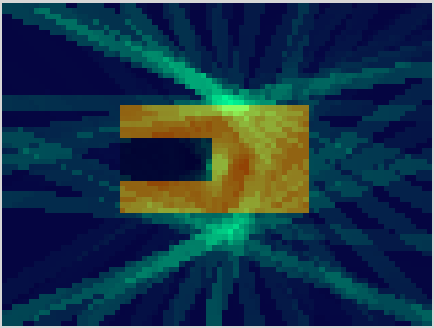
\includegraphics[scale = 0.8] {visualization3_actual.png} 
	\caption{Radiation for actual data in Task 1, Part 3}
\end{figure}

\item Implementation and visualization of the enhanced models we have come up with. 


\textbf{Minimization of Total Radiation} 

We minimize radiation over the entire region. We do this by altering our objective function in task 1.2. We take out our binary parameter and allow iteration over the entire region. 

In the small tumor case we take advantage of beams 1, 2 and 5. Compared to our result in task 1.3, we see a weakening in beam 1 from 20 to 17.6. 	

\begin{figure} [H]
	\centering
	
\includegraphics[scale = 3.0] {visualization5_rad_small.png} 
	\caption{Radiation for small data in Task 1, Part 5}
\end{figure}

\begin{figure} [H]
	\centering
	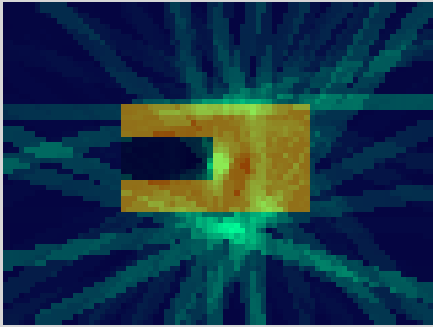
\includegraphics[scale = 0.8] {visualization5_rad_actual.png} 
	\caption{Radiation for actual data in Task 1, Part 5}
\end{figure}

\textbf{Regenerative Radiation}

Here we allow radiation or waves to be able to strengthen cells, in addition to being able to destroy them. We do this by relaxing the non-negativity constraint on our beam. 

\begin{figure} [H]
	\centering
	
\includegraphics[scale = 3.0] {visualization5_pos_small.png} 
	\caption{Radiation for small data in Task 1, Part 5}
\end{figure}

We can see how Matlab's visualization uses coloration to differentiate between positive and negative rays. 

\begin{figure} [H]
	\centering
	
\includegraphics[scale = 0.8] {visualization5_pos_actual.png} 
	\caption{Radiation for actual data in Task 1, Part 5}
\end{figure}


\end{enumerate}
\end{task}


%%%%%%%%%%%%%%%%%%%%%%%%%%%%%%%

% task 3
\begin{task}{Appendix 1: AMPL Code}
\begin{enumerate}
\item We want to show the files enumerated above (quickly again below) here:

\begin{list}{*}{}
	\item \textbf{Mod file:} bin1.mod 
	\item \textbf{Data files:} CT\_actual.dat and CT\_small.dat
	\item \textbf{Run files:} bin1.run
	\item  \textbf{Result files:} beam1\_int\_actual.txt
\end{list}

The following is the model file, bin1.mod:
\begin{lstlisting}
# Task 1, Part 1 Mod File
# Applied Mathematics 121
# David Freed, Chris Bruno, Jeremy Nixon, Millie Shi
# October 6, 2014

param num_beams;                  # number of beams

param num_rows >= 1, integer;     # number of rows
param num_cols >= 1, integer;     # number of columns 

set ROWS    := 1 .. num_rows;	  # set of rows
set COLUMNS := 1 .. num_cols;	  # set of columns
set BEAMS   := 1 .. num_beams;    # set of beams

# values for entries of each beam
param beam_values {BEAMS, ROWS, COLUMNS} >= 0; 

# values of tumor
param tumor_values {ROWS, COLUMNS} >= 0; 

# define the tumor area 
set tumor_area := {j in ROWS, k in COLUMNS: tumor_values[j,k] > 0};

# values of critical area
param critical_values {ROWS, COLUMNS} >= 0; 

# define critical area 
set critical_area := {j in ROWS, k in COLUMNS: critical_values[j,k] > 0};

# critical maximum dosage requirement
param critical_max;

# tumor minimum dosage requirement
param tumor_min;

# binary parameter for critical region and tumor region
param a {j in ROWS, k in COLUMNS} = if critical_values[j,k] > 0 then 1 else 0;
param e {j in ROWS, k in COLUMNS} = if tumor_values[j,k] > 0 then 1 else 0;

# dosage scalar of each beam
var X {i in BEAMS} >= 0;

# minimize total dosage in critical area
minimize total_critical_dosage: sum {i in BEAMS} sum {j in ROWS, k in COLUMNS} a[j,k] * X[i] * beam_values[i,j,k];

# total dosage at each tumor location [j,k] should be >= min tumor dosage with slack variable
subject to tumor_limit {j in ROWS, k in COLUMNS} : sum {i in BEAMS} X[i] * beam_values[i,j,k] >= tumor_min * e[j,k];

# total dosage at each critical location [j,k] should be <= max critical dosage with slack variable
subject to critical_limit {j in ROWS, k in COLUMNS} : sum {i in BEAMS} a[j,k] * X[i] * beam_values[i,j,k] <= critical_max;

\end{lstlisting}

We use the following for our first data file, CT\_small.dat (the small example):
\begin{lstlisting}
# Task 1, Part 1 Small Data File
# Applied Mathematics 121
# David Freed, Chris Bruno, Jeremy Nixon, Millie Shi
# October 6, 2014

param num_rows := 8;     # Number of rows
param num_cols := 8;     # Number of columns 

param num_beams := 5;    # Number of beams in small sample

param critical_max := 2;
param tumor_min := 10;

# read in beam data into 3D array beam_values, beam m
read {m in BEAMS, i in ROWS, j in COLUMNS} beam_values[m,i,j] < beam_raw_small.txt;

# read in tumor data
read {i in ROWS, j in COLUMNS} tumor_values[i,j] < tumor_raw_small.txt;

# read in critical area data
read {i in ROWS, j in COLUMNS} critical_values[i,j] < critical_raw_small.txt;
\end{lstlisting}

We use the following for our second data file, CT\_actual.dat (the large example):
\begin{lstlisting}
# Task 1, Part 1 Actual Data File
# Applied Mathematics 121
# David Freed, Chris Bruno, Jeremy Nixon, Millie Shi
# October 6, 2014

param num_rows := 60;     # Number of rows, change for big sample
param num_cols := 80;     # Number of columns 

param num_beams := 126;    # Number of beams in small sample

param critical_max := 2;
param tumor_min := 10;

# read in beam data into 3D array beam_values, beam m
read {m in BEAMS, i in ROWS, j in COLUMNS} beam_values[m,i,j] < beam_raw.txt;

# read in tumor data
read {i in ROWS, j in COLUMNS} tumor_values[i,j] < tumor_raw.txt;

# read in critical area data
read {i in ROWS, j in COLUMNS} critical_values[i,j] < critical_raw.txt;
\end{lstlisting}

The following script, bin1.run, is our run script for bin1.mod and CT\_actual.dat and CT\_small.dat.:
\begin{lstlisting}
# Task 1, Part 1 Run File
# Applied Mathematics 121
# David Freed, Chris Bruno, Jeremy Nixon, Millie Shi
# October 6, 2014

# Clear data history
reset;

# Test on small data set
model bin1.mod;
data CT_small.dat;
option solver './cplex';
solve;
display X;

# Export X as a .txt file for MATLAB code
display X > beam1_int_small.txt;

# Clear data history
reset;

# Use on actual data set
model bin1.mod;
data CT_actual.dat;
option solver './cplex';
solve;
display X;

# There is no need to export X because this is infeasible. X is an array of 0s

\end{lstlisting}

This is the output file, beam1\_int\_small.txt, that contains the dosages delivered per beam for the small matrix:

\begin{lstlisting}
X [*] :=
1  20
2  12.5
3   0
4   0
5  20
;
\end{lstlisting}

In order to use this matrix as an input in MATLAB, we edit the .txt file to look like this instead:
\begin{lstlisting}
1  20
2  12.5
3   0
4   0
5  20
\end{lstlisting}

For the actual file, we get the following output (copied-and-pasted from AMPL).

\begin{lstlisting}
ampl: solve;
presolve: constraint tumor_limit[22,41] cannot hold:
	body >= 10 cannot be <= 6.05546; difference = 3.94454
presolve: constraint tumor_limit[23,41] cannot hold:
	body >= 10 cannot be <= 6.00316; difference = 3.99684
presolve: constraint tumor_limit[23,42] cannot hold:
	body >= 10 cannot be <= 5.69247; difference = 4.30753
presolve: constraint tumor_limit[24,42] cannot hold:
	body >= 10 cannot be <= 5.71775; difference = 4.28225
presolve: constraint tumor_limit[38,39] cannot hold:
	body >= 10 cannot be <= 7.91302; difference = 2.08698
229 presolve messages suppressed.
ampl: display X;
X [*] :=
  1 0    14 0    27 0    40 0    53 0    66 0    79 0    92 0   105 0   118 0
  2 0    15 0    28 0    41 0    54 0    67 0    80 0    93 0   106 0   119 0
  3 0    16 0    29 0    42 0    55 0    68 0    81 0    94 0   107 0   120 0
  4 0    17 0    30 0    43 0    56 0    69 0    82 0    95 0   108 0   121 0
  5 0    18 0    31 0    44 0    57 0    70 0    83 0    96 0   109 0   122 0
  6 0    19 0    32 0    45 0    58 0    71 0    84 0    97 0   110 0   123 0
  7 0    20 0    33 0    46 0    59 0    72 0    85 0    98 0   111 0   124 0
  8 0    21 0    34 0    47 0    60 0    73 0    86 0    99 0   112 0   125 0
  9 0    22 0    35 0    48 0    61 0    74 0    87 0   100 0   113 0   126 0
 10 0    23 0    36 0    49 0    62 0    75 0    88 0   101 0   114 0
 11 0    24 0    37 0    50 0    63 0    76 0    89 0   102 0   115 0
 12 0    25 0    38 0    51 0    64 0    77 0    90 0   103 0   116 0
 13 0    26 0    39 0    52 0    65 0    78 0    91 0   104 0   117 0
;
\end{lstlisting}

\item We want to update the initial model for the changes made in Task 1, Part 2. We do not have to change the data files for this so we use the following files:

\begin{list}{*}{}
	\item \textbf{Mod file:} bin2.mod 
	\item \textbf{Data files:} CT\_actual.dat and CT\_small.dat
	\item \textbf{Run files:} bin2.run
	\item  \textbf{Result files:} beam2\_int\_actual.txt
\end{list}

We will not reprint the data files since they are unchanged. The following is the model file, bin2.mod:

\begin{lstlisting}
param num_beams;                  # number of beams

param num_rows >= 1, integer;     # number of rows
param num_cols >= 1, integer;     # number of columns 

set ROWS    := 1 .. num_rows;	  # set of rows
set COLUMNS := 1 .. num_cols;	  # set of columns
set BEAMS   := 1 .. num_beams;    # set of beams

# values for entries of each beam
param beam_values {BEAMS, ROWS, COLUMNS} >= 0; 

# values of tumor
param tumor_values {ROWS, COLUMNS} >= 0; 

# define the tumor area 
set tumor_area := {j in ROWS, k in COLUMNS: tumor_values[j,k] > 0};

# values of critical area
param critical_values {ROWS, COLUMNS} >= 0; 

# define critical area 
set critical_area := {j in ROWS, k in COLUMNS: critical_values[j,k] > 0};

# critical maximum dosage requirement
param critical_max;

# tumor minimum dosage requirement
param tumor_min;

# binary parameter for critical region and tumor region
param a {j in ROWS, k in COLUMNS} = if critical_values[j,k] > 0 then 1 else 0;
param e {j in ROWS, k in COLUMNS} = if tumor_values[j,k] > 0 then 1 else 0;

# dosage scalar of each beam
var X {i in BEAMS} >= 0;

# slack variables
var S {j in ROWS, k in COLUMNS} >= 0;
var T {j in ROWS, k in COLUMNS} >= 0;

# minimize total dosage in critical area
minimize total_critical_dosage: sum {j in ROWS, k in COLUMNS} (S[j,k] + T[j,k]);

# total dosage at each tumor location [j,k] should be >= min tumor dosage with slack variable
subject to tumor_limit {j in ROWS, k in COLUMNS} : sum {i in BEAMS} X[i] * beam_values[i,j,k] * e[j,k] >= (tumor_min - T[j,k]) * e[j,k] ;

# total dosage at each critical location [j,k] should be <= max critical dosage with slack variable
subject to critical_limit {j in ROWS, k in COLUMNS} : sum {i in BEAMS} a[j,k] * X[i] * beam_values[i,j,k] <= critical_max + S[j,k];
\end{lstlisting}

The following script is our run script for bin2.mod and CT\_actual.dat and CT\_small.dat:
\begin{lstlisting}
# Task 1, Part 2 Run File
# Applied Mathematics 121
# David Freed, Chris Bruno, Jeremy Nixon, Millie Shi
# October 6, 2014

# Clear data history
reset;

# Test on small data set
model bin2.mod;
data CT_small.dat;
option solver './cplex';
solve;
display X;

# No need to export X because it is the same as beam1_int_small.txt

# Clear data history
reset;

# Use on actual data set
model bin2.mod;
data CT_actual.dat;
option solver './cplex';
solve;
display X;

# Export X as a .txt file for the MATLAB code:
display X > beam2_int_actual.txt;
\end{lstlisting}

The previous output file, beam1\_int\_small.txt, contains the dosages delivered per beam for the small matrix. We have to make no changes to this because the optimal solution is the same, as shown below:

\begin{lstlisting}
X [*] :=
1  20
2  12.5
3   0
4   0
5  20
;
\end{lstlisting}

The following output file, beam2\_int\_small.txt, contains the dosages delivered per beam for the actual matrix, now that we have a feasible solution:

\begin{lstlisting}
X [*] :=
  1  0            33  5.56661      65  0            97  0
  2  0            34  6.66667      66 12.3129       98  0.948631
  3 14.2907       35 13.1579       67  0            99  9.75368
  4  0.537311     36  0.673964     68  0           100  0
  5 15.625        37  6.66667      69  0           101  0
  6  0            38  0            70  0           102  0
  7  0            39  0            71  0           103  0
  8  0            40 10.6478       72  0           104 10.0882
  9 13.2165       41  0            73  0           105  1.10485
 10  0            42  0.809229     74  0           106  0
 11  8.10364      43  4.85492      75  0           107  0
 12  0            44  0.259757     76  0           108  0
 13  0            45  0            77  1.53722     109  0
 14  0.176443     46  1.23007      78  0           110  0
 15 11.5073       47  0            79  0           111  0.221729
 16  2.20913      48  1.0365       80  0.137174    112  0
 17 13.5135       49  4.32929      81  0           113  0
 18  0            50  0.242279     82  0           114  0
 19  0            51  0            83 15.0284      115  1.33431
 20  0.124556     52  0            84  0           116  0
 21 11.4565       53  0            85  0           117  0
 22  1.38967      54  1.161        86  0.956878    118  0
 23  1.8792       55  0            87 11.1841      119  0
 24  0.219834     56  0            88  0           120  0
 25  1.86593      57  0            89  0           121  5.72499
 26  0.0134325    58  9.77891      90  0           122  0
 27  6.18207      59  0            91  0           123  0
 28  0.0938967    60  0.0121859    92 10.5779      124  0.36483
 29  9.42494      61  0.332151     93  0           125  0
 30  0.827491     62  0            94  0           126  0
 31  0            63  0            95  0
 32  0            64  0.166218     96  0
;
\end{lstlisting}


\item We now update the initial model for the changes made in Task 1, Part 3. We do not have to change the data files once again. We are using the following files:

\begin{list}{*}{}
	\item \textbf{Mod file:} bin3.mod 
	\item \textbf{Data files:} CT\_actual.dat and CT\_small.dat
	\item \textbf{Run files:} bin3.run
	\item  \textbf{Result files:} beam3\_int\_actual.txt and beam3\_int\_small.txt
\end{list}

We will again not reprint the data files since they are unchanged. The following is the model file, bin3.mod:

\begin{lstlisting}
param num_beams;                  # number of beams

param num_rows >= 1, integer;     # number of rows
param num_cols >= 1, integer;     # number of columns 

set ROWS    := 1 .. num_rows;	  # set of rows
set COLUMNS := 1 .. num_cols;	  # set of columns
set BEAMS   := 1 .. num_beams;    # set of beams

# values for entries of each beam
param beam_values {BEAMS, ROWS, COLUMNS} >= 0; 

# values of tumor
param tumor_values {ROWS, COLUMNS} >= 0; 

# define the tumor area 
set tumor_area := {j in ROWS, k in COLUMNS: tumor_values[j,k] > 0};

# values of critical area
param critical_values {ROWS, COLUMNS} >= 0; 

# define critical area 
set critical_area := {j in ROWS, k in COLUMNS: critical_values[j,k] > 0};

# critical maximum dosage requirement
param critical_max;

# tumor minimum dosage requirement
param tumor_min;

# binary parameter for critical region and tumor region
param a {j in ROWS, k in COLUMNS} = if critical_values[j,k] > 0 then 1 else 0;
param e {j in ROWS, k in COLUMNS} = if tumor_values[j,k] > 0 then 1 else 0;

# dosage scalar of each beam
var X {i in BEAMS} >= 0;

# slack variables
var S {j in ROWS, k in COLUMNS} >= 0;
var T {j in ROWS, k in COLUMNS} >= 0;

# minimize total dosage in critical area
minimize total_critical_dosage: sum {j in ROWS, k in COLUMNS} ( (S[j,k] + T[j,k]) + sum {i in BEAMS} sum {m in -1 .. 1} sum {n in -1 .. 1} (1 - a[j,k]) * (a[min(max(j+m,1), num_rows),min(max(k+n,1),num_cols)]) * X[i] * beam_values[i,j,k]);

# total dosage at each tumor location [j,k] should be >= min tumor dosage with slack variable
subject to tumor_limit {j in ROWS, k in COLUMNS} : sum {i in BEAMS} X[i] * beam_values[i,j,k] * e[j,k] >= (tumor_min - T[j,k]) * e[j,k] ;

# total dosage at each critical location [j,k] should be <= max critical dosage with slack variable
subject to critical_limit {j in ROWS, k in COLUMNS} : sum {i in BEAMS} a[j,k] * X[i] * beam_values[i,j,k] <= critical_max + S[j,k];
\end{lstlisting}

The following script is our run script for bin3.mod and CT\_actual.dat and CT\_small.dat:

\begin{lstlisting}
# Task 1, Part 3 Run File
# Applied Mathematics 121
# David Freed, Chris Bruno, Jeremy Nixon, Millie Shi
# October 6, 2014

# Clear data history
reset;

# Test on small data set
model bin3.mod;
data CT_small.dat;
option solver './cplex';
solve;
display X;

# Export X as a .txt file for the MATLAB code:
display X > beam3_int_small.txt;

# Clear data history
reset;

# Use on actual data set
model bin3.mod;
data CT_actual.dat;
option solver './cplex';
solve;
display X;


# Export X as a .txt file for the MATLAB code:
display X > beam3_int_actual.txt;
\end{lstlisting}

Below are the output files for the two situations. The first is the small data set, where we can see that we optimize at values that are different than in the previous two problems:

\begin{lstlisting}
X [*] :=
1   0
2   0
3   0
4   0
5  20
;
\end{lstlisting}

The second is for the actual data set, where we have different optimal values than before:

\begin{lstlisting}
X [*] :=
  1  0            33 12.5082       65  0            97  0
  2  0            34  0.338356     66  0.352361     98 12.6267
  3 15.625        35 13.1579       67  0            99  2.24737
  4  0            36  0            68  0           100  0
  5 15.625        37  0            69  0           101  0
  6  0            38  0            70  0           102  0
  7  0            39  0            71  0           103  0
  8  0            40  2.77778      72  0           104 11.6279
  9 14.4928       41  0            73  0           105  0
 10  0.316385     42  0.102634     74  0           106  0
 11 13.6527       43 12.5082       75  0           107  0
 12  0            44  0            76  0           108  0
 13  0            45  0            77 12.218       109  0
 14  0            46  0            78  0           110  0
 15 12.8127       47  0            79  0           111  0
 16  0            48  0.0947393    80  0           112  0
 17 13.5135       49  0            81  0           113  0
 18  0            50  0            82  0           114  0
 19  0            51  0            83  4.76053     115  0
 20  0            52  0            84  0           116  0
 21 12.7949       53  0            85  0           117  0
 22  0            54  0            86  0           118  0
 23  0.656476     55  0            87 11.8241      119  0
 24  0            56  0            88  0           120  0
 25  0            57  0            89  0           121  0
 26  0            58  0            90  0           122  0
 27  0.633051     59  0            91  0           123  0
 28  0            60  0            92  0           124  0
 29 12.3457       61  0            93  8.18031     125  0
 30  0            62  0            94  0           126  0
 31  0            63  0            95  0
 32  2.53165      64  0            96  0
;
\end{lstlisting}

\item We will now change the files substantially to adjust for our enhancements. For our first enhancement, we are using the following files:

\begin{list}{*}{}
	\item \textbf{Mod file:} t5\_pos.mod 
	\item \textbf{Data files:} CT\_actual.dat and CT\_small.dat
	\item \textbf{Run files:} t5.run
	\item  \textbf{Result files:} beam5\_rad\_int\_actual.txt and beam5\_rad\_int\_small.txt
\end{list}

For the second enhancement, we are using the following files:

\begin{list}{*}{}
	\item \textbf{Mod file:} t5\_pos.mod 
	\item \textbf{Data files:} CT\_actual.dat and CT\_small.dat
	\item \textbf{Run files:} t5.run
	\item  \textbf{Result files:} beam5\_pos\_int\_actual.txt and beam5\_pos\_int\_small.txt
\end{list}

The first enhancement has the .mod file t5\_pos.mod:

\begin{lstlisting}
param num_beams;                  # number of beams

param num_rows >= 1, integer;     # number of rows
param num_cols >= 1, integer;     # number of columns 

set ROWS    := 1 .. num_rows;	  # set of rows
set COLUMNS := 1 .. num_cols;	  # set of columns
set BEAMS   := 1 .. num_beams;    # set of beams

# values for entries of each beam
param beam_values {BEAMS, ROWS, COLUMNS} >= 0; 

# values of tumor
param tumor_values {ROWS, COLUMNS} >= 0; 

# define the tumor area 
set tumor_area := {j in ROWS, k in COLUMNS: tumor_values[j,k] > 0};

# values of critical area
param critical_values {ROWS, COLUMNS} >= 0; 

# define critical area 
set critical_area := {j in ROWS, k in COLUMNS: critical_values[j,k] > 0};

# critical maximum dosage requirement
param critical_max;

# tumor minimum dosage requirement
param tumor_min;

# binary parameter for critical region and tumor region
param a {j in ROWS, k in COLUMNS} = if critical_values[j,k] > 0 then 1 else 0;
param e {j in ROWS, k in COLUMNS} = if tumor_values[j,k] > 0 then 1 else 0;

# dosage scalar of each beam
var X {i in BEAMS};

# slack variables
var S {j in ROWS, k in COLUMNS} >= 0;
var T {j in ROWS, k in COLUMNS} >= 0;

# minimize total dosage in critical area
minimize total_critical_dosage: sum {j in ROWS, k in COLUMNS} (10 * (S[j,k] + T[j,k]) + sum {i in BEAMS} sum {m in -1 .. 1} sum {n in -1 .. 1} e[j,k] * a[min(max(j+m,1), num_rows),min(max(k+n,1),num_rows)] * X[i] * beam_values[i,j,k]);

# total dosage at each tumor location [j,k] should be >= min tumor dosage with slack variable
subject to tumor_limit {j in ROWS, k in COLUMNS} : sum {i in BEAMS} X[i] * beam_values[i,j,k] * e[j,k] >= (tumor_min - T[j,k]) * e[j,k] ;

# total dosage at each critical location [j,k] should be <= max critical dosage with slack variable
subject to critical_limit {j in ROWS, k in COLUMNS} : sum {i in BEAMS} a[j,k] * X[i] * beam_values[i,j,k] <= critical_max + S[j,k];
\end{lstlisting}

The second enhancement has the .mod file t5\_rad.mod:

\begin{lstlisting}
param num_beams;                  # number of beams

param num_rows >= 1, integer;     # number of rows
param num_cols >= 1, integer;     # number of columns 

set ROWS    := 1 .. num_rows;	  # set of rows
set COLUMNS := 1 .. num_cols;	  # set of columns
set BEAMS   := 1 .. num_beams;    # set of beams

# values for entries of each beam
param beam_values {BEAMS, ROWS, COLUMNS} >= 0; 

# values of tumor
param tumor_values {ROWS, COLUMNS} >= 0; 

# define the tumor area 
set tumor_area := {j in ROWS, k in COLUMNS: tumor_values[j,k] > 0};

# values of critical area
param critical_values {ROWS, COLUMNS} >= 0; 

# define critical area 
set critical_area := {j in ROWS, k in COLUMNS: critical_values[j,k] > 0};

# critical maximum dosage requirement
param critical_max;

# tumor minimum dosage requirement
param tumor_min;

# binary parameter for critical region and tumor region
param a {j in ROWS, k in COLUMNS} = if critical_values[j,k] > 0 then 1 else 0;
param e {j in ROWS, k in COLUMNS} = if tumor_values[j,k] > 0 then 1 else 0;

# dosage scalar of each beam
var X {i in BEAMS} >= 0;

# slack variables
var S {j in ROWS, k in COLUMNS} >= 0;
var T {j in ROWS, k in COLUMNS} >= 0;

# minimize total dosage in critical area
minimize total_critical_dosage: sum {j in ROWS, k in COLUMNS} (100 * (S[j,k] + T[j,k]) + sum {i in BEAMS} (e[j,k] + a[j,k]) * X[i] * beam_values[i,j,k]);

# total dosage at each tumor location [j,k] should be >= min tumor dosage with slack variable
subject to tumor_limit {j in ROWS, k in COLUMNS} : sum {i in BEAMS} X[i] * beam_values[i,j,k] * e[j,k] >= (tumor_min - T[j,k]) * e[j,k] ;

# total dosage at each critical location [j,k] should be <= max critical dosage with slack variable
subject to critical_limit {j in ROWS, k in COLUMNS} : sum {i in BEAMS} a[j,k] * X[i] * beam_values[i,j,k] <= critical_max + S[j,k];
\end{lstlisting}

The run file works on both enhancements:

\begin{lstlisting}
# Task 1, Part 5 Run File
# Applied Mathematics 121
# David Freed, Chris Bruno, Jeremy Nixon, Millie Shi
# October 6, 2014

# Clear data history
reset;

# Test rad enhancement on small data set
model t5_rad.mod;
data CT_small.dat;
option solver './cplex';
solve;
display X;

# Export X as a .txt file for the MATLAB code:
display X > beam5_rad_int_small.txt;

# Clear data history
reset;

# Test rad enhancement on actual data set
model t5_rad.mod;
data CT_actual.dat;
option solver './cplex';
solve;
display X;

# Export X as a .txt file for the MATLAB code:
display X > beam5_rad_int_actual.txt;

# Clear data history
reset;

# Test pos enhancement on small data set
model t5_pos.mod;
data CT_small.dat;
option solver './cplex';
solve;
display X;

# Export X as a .txt file for the MATLAB code:
display X > beam5_pos_int_small.txt;

# Clear data history
reset;

# Test pos enhancement on actual data set
model t5_pos.mod;
data CT_actual.dat;
option solver './cplex';
solve;
display X;

# Export X as a .txt file for the MATLAB code:
display X > beam5_pos_int_actual.txt;
\end{lstlisting}

The following output file works for the first enhancement on the small matrix:
\begin{lstlisting}
X[*] :=
1   17.6
2   60.4615
3  -76.7385
4    2
5   22.4
;
\end{lstlisting}

The following output file works for the first enhancement on the actual matrix:
\begin{lstlisting}
X[*] !=
  1   -33.3754       33     6.75384      65     0            97 -2655.74
  2  -177.113        34     0.478014     66     1.21149      98    63.1373
  3   872.74         35    -8.68387      67   -23.288        99    32.6798
  4   -96.853        36    15.337        68   186.618       100  2706.87
  5   407.225        37     7.9022       69     0           101     0
  6   -20.1545       38    25.8173       70   108.555       102     0
  7  -419.902        39     0            71     0           103  -176.993
  8   -14.5876       40     6.71141      72     0           104    -1.67839
  9   723.038        41     0            73   -32.8652      105   -28.1587
 10   -43.5652       42     4.3601       74   -17.9313      106   372.154
 11    60.1144       43     0.440813     75     0           107     0
 12    10.3138       44     9.01493      76     3.84417     108     0
 13    -8.56901      45     0            77    78.4416      109    41.9914
 14     5.65578      46    61.4255       78     0           110     0
 15    67.3655       47     0            79  -135.361       111    11.2741
 16    -3.89297      48     7.60956      80    -5.01985     112    10.5846
 17    62.0808       49    11.494        81  -798.418       113     0
 18    12.4151       50    12.1508       82     5.81053     114     0
 19   -55.9827       51     0            83   687.507       115    -7.97999
 20    -9.58734      52     8.53895      84     0           116     0
 21    53.4657       53     0            85   -52.8811      117    18.573
 22    -0.0321426    54     1.84348      86    28.2378      118   144.458
 23   -47.3679       55    51.8845       87    54.7066      119     0
 24    -8.22184      56    59.9723       88   -59.1823      120     0
 25     0.484152     57     0            89     0           121     1.07008
 26    -7.35098      58   456.234        90     0           122     0
 27    22.861        59     0            91  -362.559       123     5.3649
 28     4.85277      60    14.2607       92    13.91        124    17.9472
 29   814.844        61    -7.69532      93  -112.977       125     0
 30     2.05653      62     1.26625      94   172.358       126     0
 31     6.22726      63     0            95     0
 32     8.62331      64    31.122        96     0
;
\end{lstlisting}

The following output file works for the second enhancement on the small matrix:
\begin{lstlisting}
X[*] :=
1  20
2  12.5
3   0
4   0
5  20
;
\end{lstlisting}

The following output file works for the second enhancement on the actual matrix:
\begin{lstlisting}
X[*] :=
  1  0            33  5.41257      65  3.68532      97  0
  2  0            34  6.75453      66  0            98  0.912308
  3  0            35  4.4772       67  0            99  9.57952
  4  1.48156      36  0.880286     68  0           100  0
  5  1.8845       37  6.49789      69  0           101  2.79121
  6  0            38  0            70  0           102  0
  7  0            39  0            71  0           103  0
  8  0            40  7.76236      72  0           104  0
  9  3.00704      41  8.68069      73  0.531535    105  1.33001
 10  0            42  0.860362     74  0           106  0
 11 10.229        43  5.16435      75  0           107  0.500962
 12  0.0191044    44  0.312712     76  0           108  0
 13  0            45  0            77  1.93674     109  0
 14  0.291983     46  1.11264      78  0           110  0
 15  0            47  0            79  0           111  0.0197262
 16  1.98307      48  0.88271      80  0.136182    112  0
 17  1.25856      49  4.28363      81  0           113  0
 18  0            50  0.303063     82  0           114  1.00251
 19  0            51  1.06525      83  0.0174297   115  1.19548
 20  0            52  0            84  0           116 11.1859
 21  1.89942      53  1.07851      85  0           117  0
 22  1.18864      54  1.13408      86  0.919641    118  0
 23  1.13435      55  0            87  0           119  0
 24  0.295085     56  0            88  0           120  0
 25  4.27168      57  8.47205      89 14.5275      121  4.98328
 26  0            58  7.38601      90  0           122  0
 27  0.53074      59  2.01847      91  0           123  0
 28  0.204438     60  0.023738     92 10.5434      124  0
 29  7.51516      61  0.416096     93  0           125  0
 30  0.630934     62  0            94  0           126 12.4646
 31  0.0628224    63  8.51983      95  0
 32  0            64  0            96  0
;
\end{lstlisting}

\end{enumerate}
\end{task}

\end{document}

